\documentclass[12pt]{article}
\textwidth 16.5cm
\textheight 23.5cm
\oddsidemargin 0pt
\topmargin -2cm
\usepackage{epsf}
%\usepackage{enumerate}
%\usepackage{url} % not crucial - just used below for the URL 

%\pdfminorversion=4
% NOTE: To produce blinded version, replace "0" with "1" below.



%\setlength{\parindent}{.3in}
%\setlength{\parskip}{.05in}
\usepackage{natbib}
\usepackage{latexsym,amsmath,amssymb,amsfonts,amsthm,bbm,mathrsfs,breakcites, dsfont,xcolor}
\usepackage{stmaryrd,epsf}
\usepackage{soul}
\usepackage{url}
\usepackage{dsfont}
\usepackage{enumerate}
\usepackage{enumitem}   
\usepackage{graphicx}
\usepackage{graphics}
\usepackage{psfrag}
\usepackage{caption, subcaption}
%\usepackage{algorithm}
\usepackage[ruled,vlined]{algorithm2e}

%\usepackage{comment}
%\newcommand{\indep}{\rotatebox[origin=c]{90}{$\models4[]}
\usepackage[colorlinks,linkcolor=black,citecolor=black,urlcolor=blue,breaklinks = true]{hyperref}

\newtheorem{theorem}{Theorem}
\newtheorem{lemma}[theorem]{Lemma}
%\newtheorem{example}[]{Example}
\newtheorem{proposition}[theorem]{Proposition}
\newtheorem{corollary}[theorem]{Corollary}
\newtheorem{assumption}{A\!\!}
\newtheorem{example}{Example}
% \renewcommand{\baselinestretch}{1.25}
\newcommand{\indep}{\rotatebox[origin=c]{90}{$\models$}}
\newcommand{\red}[1]{\textcolor{red}{#1}}
\newcommand{\blue}[1]{\textcolor{blue}{#1}}
\newcommand{\green}[1]{\textcolor{green}{#1}}
\newcommand{\orange}[1]{\textcolor{orange}{#1}}
\newcommand{\var}{\mathrm{Var}}
\newcommand{\cov}{\mathrm{Cov}}
\newcommand{\bbE}{\mathbb{E}}

% Keywords command
\providecommand{\keywords}[1]
{
  \small	
  \textbf{Keywords:} #1
}


\DeclareMathOperator*{\argmin}{argmin}
\DeclareMathOperator*{\argmax}{argmax}
\DeclareMathOperator*{\sargmin}{sargmin}
\DeclareMathOperator*{\sargmax}{sargmax}



\newenvironment{definition}[1][Definition]{\begin{trivlist}
\item[\hskip \labelsep {\bfseries #1}]}{\end{trivlist}}
\newenvironment{remark}[1][Remark.]{\begin{trivlist}
\item[\hskip \labelsep {\bfseries #1}]}{\end{trivlist}}

\usepackage{xcolor}
\usepackage[draft,inline,nomargin,index]{fixme}
\fxsetup{theme=color,mode=multiuser}
\FXRegisterAuthor{jb}{ajb}{\color{blue} jb}
\FXRegisterAuthor{tc}{atc}{\color{red} TC}


\usepackage[acronym, toc]{glossaries-extra}

\setabbreviationstyle[acronym]{long-short}

\glssetcategoryattribute{acronym}{nohyperfirst}{true}

\renewcommand*{\glsdonohyperlink}[2]{%
 {\glsxtrprotectlinks \glsdohypertarget{#1}{#2}}}
 
\makeglossaries 

\newacronym{sdr}{SDR}{Supervised Dimensionality Reduction}

\title{Supervised Dimensionality Reduction with Random Projection-Based Ensemble Learning}
\author{Jacob R. Bradley, Timothy I. Cannings}
\date{}

\setcitestyle{authoryear, open={(},close={)}}


\begin{document}

\maketitle

\begin{abstract}
We propose a class of algorithms for \glsxtrlong{sdr} based on ensembles of random projections coupled with a low-dimensional classifier. Our core method is agnostic to the learning procedure employed, and can produce informative representations for a variety of high-dimensional data types.
\end{abstract}

\section{Introduction}
\gls{sdr} entails producing low-dimensional representations of high-dimensional objects, which preserve information with respect to a target variable. Applications of \gls{sdr} are found in data compression, visualisation, and as a pre-training step for further predictive models. We propose a class of algorithms for \gls{sdr} based on ensembles of random projections coupled with a low-dimensional classifier. Our core method is agnostic to the learning procedure employed, and can produce informative representations for a variety of high-dimensional data types.

\subsection{Terminology and Basic Concepts}
We will be discussing supervised classification methods. By supervised, we mean that we are presented with labelled training data 
\[ \mathcal{T}_n = \{(x_1, y_1), (x_2, y_2), \dots, (x_n, y_n) \ | \ x_i \in \mathcal{X}, y_i \in \mathcal{Y}\}. \]
We refer to $\mathcal{X}$ as the 'input space' or 'observation space', and will assume it is a subset of real Euclidean space so that $\mathcal{X} \subset \mathbb{R}^p$. We refer to $\mathcal{Y}$ as the 'outcome space' or 'label space', and assume for simplicity that $\mathcal{Y} = \{0,1\}$. The elements of $\mathcal{T}_n$ can be considered as observations of a random variable $(X,Y)$ from a joint probability distribution $P_{X \times Y}$, although in some circumstances it will be more convenient to think of the values $x_i$ as fixed. We define a classifier as a measurable function $C: \mathcal{X} \rightarrow \mathcal{Y}$, and denote by $\mathcal{C}_{\mathcal{X},\mathcal{Y}}$ the space of all such functions (note that this is identical for regression apart from the set $\mathcal{Y}$ and the measure used). A learning procedure is a function $L : \mathcal(\mathcal{X} \times \mathcal{Y})^n \rightarrow \mathcal{C}_{\mathcal{X},\mathcal{Y}}$, i.e. a map from training data sets to classifiers. When the learning procedure used is clear (or irrelevant) we will write $C_{\mathcal{T}_n} = L(\mathcal{T}_n)$ to refer to a classifier trained on the given training data. Common learning procedures for classification include linear and quadratic discriminant analysis, $k$-nearest neighbours, logistic regression, support vector machines and random forests. 

We can measure the performance of a classifier via its risk, given by 
\[R(C) = \mathbb{E}_{(X,Y)}[\mathbbm{1}_{\{C(X) \neq Y\}}] \quad \Big( = \int_{\mathcal{X}\times \mathcal{Y}} \mathbbm{1}_{\{C(X) \neq Y\}} dP_{X\times Y}\Big).\]
Note that this definition has a close analogy with regression risk, in which the discrete distance $\mathbbm{1}_{\{C(X) \neq Y \}}$ is replaced by the $L_2$ distance $||C(X)-Y||_2^2$. In practice the quantity $R(C)$ is often intractable, and we have to estimate it with a random variable $\hat{R}$. Choices for $\hat{R}$ include the training error $\hat{R}(C) := \frac{1}{n}\sum_{(x,y) \in \mathcal{T}_n} \mathbbm{1}_{\{C(x) \neq y\}}$, or the test error 
\[\hat{R}(C) = \frac{1}{m} \sum_{(x,y) \in \mathcal{T}_{m}} \mathbbm{1}_{\{C(x) \neq y\}},\] 
where unseen observation-outcome pairs come from a second dataset $\mathcal{T}_{m} = \{(x_i, y_i) \ | \ 1 \leq i \leq m \}$.

All of the methods mentioned above suffer from a phenomenon known as the curse of dimensionality when $p$ is large \citep{mai_review_2013}. Loosely put, the curse of dimensionality refers to the observation that the volume of a region of space (such as a hypercube) increases exponentially with $p$, necessitating an exponential increase in sample size to maintain the same density of observations and so predictive performance. This is true even when dimensionality $p$ and sample size $n$ increase together at the same rate with $p<n$ (for a thorough treatment see \citet{wainwright_high-dimensional_2019}), but is particularly exacerbated when $p \gg n$. In this regime overfitting becomes very difficult to manage. In this situation it is common to make some assumption of lower dimensional structure. Common practices for imposing lower dimensional structure include sample clustering and variable selection. Both can be implemented in a variety of ways and are liable to fail in certain situations, as we shall discuss in the next section.

\subsection{Dimension Reduction and Variable Selection}
Discovering a low-dimensional structure to a high-dimensional dataset is extremely helpful for producing good classifiers, but is also a valuable goal in its own right: low-dimensional representations of data are often very useful for interpretation and visualisation in their own right. One approach is to apply a clustering procedure to the observation data (without consideration of the associated labels). This can be done using a variety of methods such as Principal Component Analysis (PCA) and t-SNE. While clustering in this way has been extremely useful for a variety of applications, there is often no \textit{a priori} reason to assume that the directions of greatest variation in a dataset will necessarily correspond to the direct of greatest variation of the response variable. As an illustration of this principle, consider subplots \textbf{A} and \textbf{B} in Figure \ref{fig:examplefigures}. For simplicity we observations with only two components, but it is easy to see how these patterns could be embedde into higher dimensional spaces. Subplot \textbf{A} illustrates the ideal configuration for pre-processing dimensionality reduction: the direction of greatest variation aligns perfectly with the direction encoding the most information about the label. Situations that look like this, broadly speaking, are very accommodating to clustering via PCA followed by learning of a lower dimensional (in this case one-dimensional) classifier. An obvious counterexample to this trend is given in subplot \textbf{B}: here this is a clear principal component and a clear direction encodintg all available information about the label, but they are not at all aligned. Were we to extract a one-dimensional subspace via PCA here, we would observe no clear pattern with respect to our label of interest. 

Another broad class of dimensionality reduction techniques can be grouped under the banner of variable selection. These include methods based on model comparison statistics (e.g. Aikake Information Criterion, Bayesian Information Criterion), sparsity-enforcing regularisation (e.g. Lasso) and stability selection. These are, broadly speaking, motivated by the assumption that there exists some subset $S^* \subset \{1,\dots,p\}$ of the components of the input space $\mathcal{X}$ containing all available information about the labels. The output of such methods will typically be a set $\bar{S}$ estimating $S^*$. These methods perform well when the true lower-dimensional structure of the data aligns well with the axes of the observation space, but are not rotationally invariant. Lower dimensional structure along any other direction may not be well expressed via projection to some subset of axes, as illustrated in subplot $\textbf{C}$. This issue becomes more severe with higher dimensionality. Finally, both of the properties discussed may be true as illustrated in \textbf{D}. In this example, while a clear one dimensional structure exists, even embedded in two dimensions no combination of clustering and variable selection will provide a good lower-dimensional representation. 

\begin{figure}[htbp]
\centering
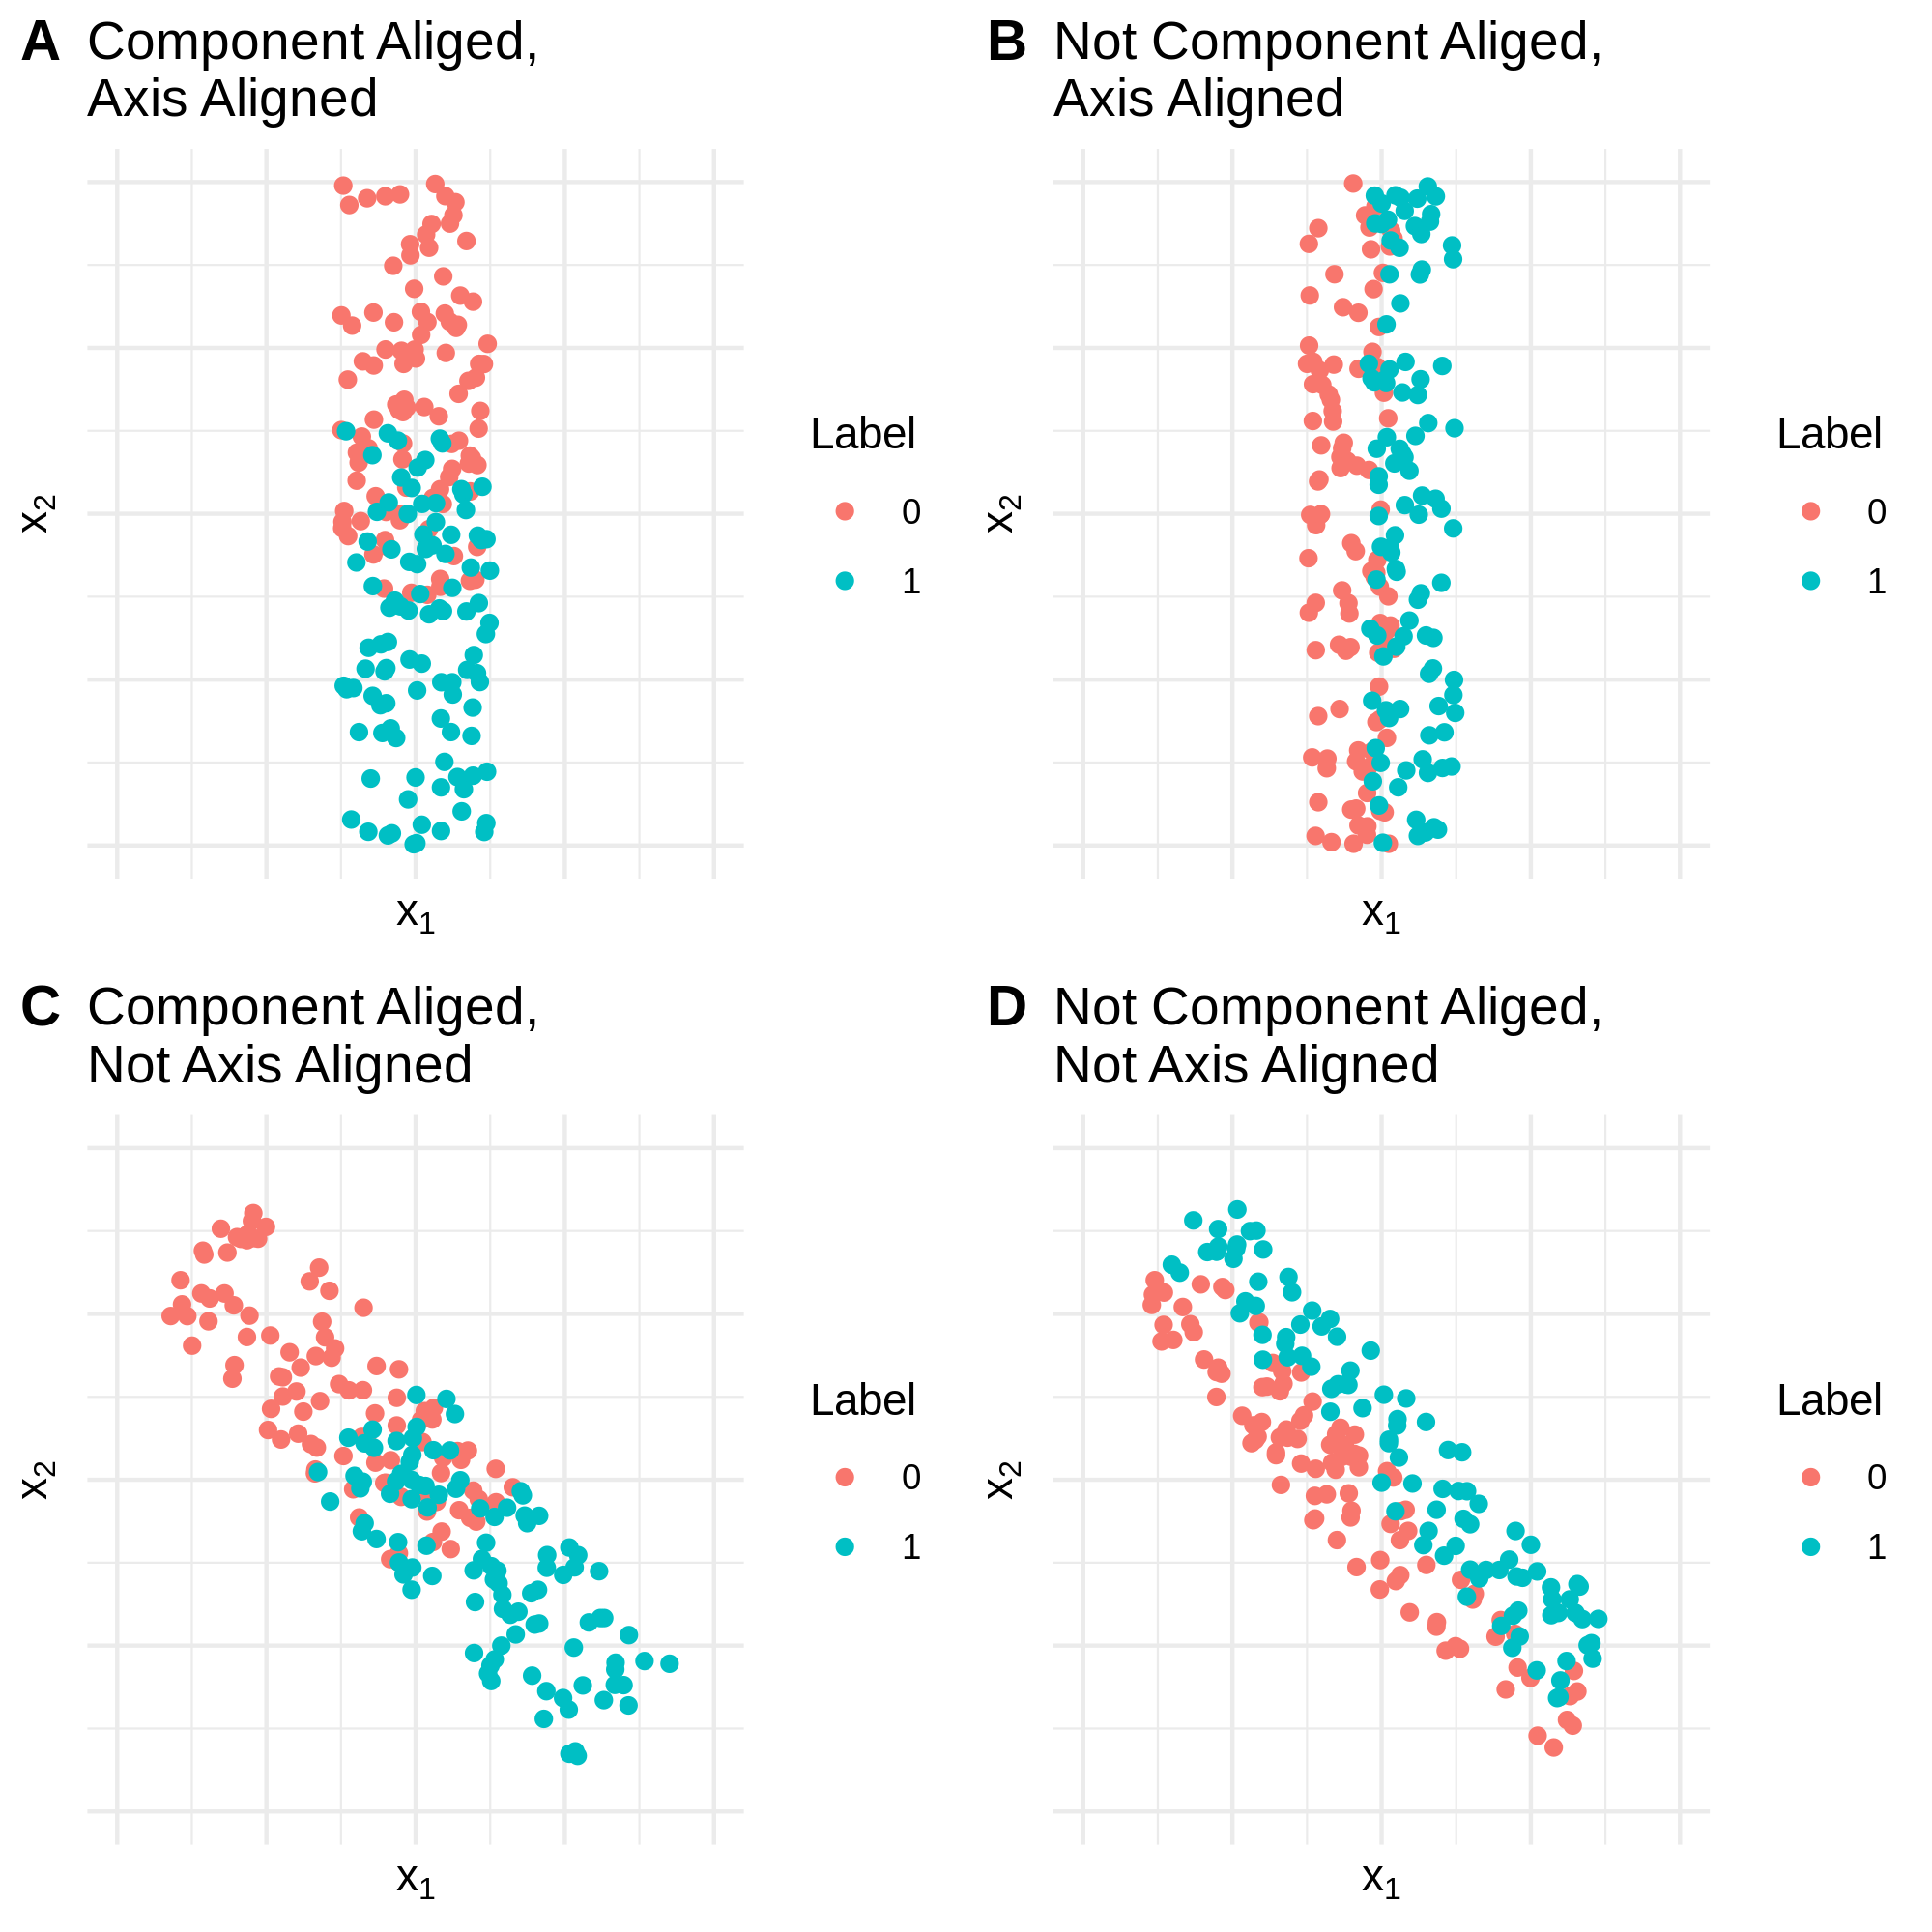
\includegraphics[width=4in]{figures/ExampleFigures.png}
\caption{Simple distributions that will provide a range of challenges to clustering and/or variable selection methods when embedded in higher dimensional space.\label{fig:examplefigures}}
\end{figure}

\subsection{Sufficient  and Central Subspaces}
In order to address the issues established in the previous section, we seek a notion of dimensionality reduction that is \textit{a)} informed by labels as well as observations and \textit{b)} rotationally invariant. To this end we consider subspace selection as a generalisation of variable selection. Intuitively, we seek a low-dimensional subspace $V \subset \mathcal{X}$ such that almost all information pertaining to label value is encapsulated by an observation's projection onto $V$. If $V$ can be expressed as the span of canonical basis (i.e. axis-aligned) vectors, then this is equivalent to variable selection. 

\begin{definition}
\textit{Sufficient Subspace}: Given random variables $X$, $Y$ drawn from a joint distribution $P_{X\times Y}$ on $\mathcal{X} \times \mathcal{Y}$, we say that there exists a sufficient subspace of dimension $d$ if there exists a projection $A : \mathbb{R}^p \rightarrow \mathbb{R}^d $ such that 

\[
X \perp\!\!\!\perp Y\ | \ AX
\]
where $A$ being a projection mandates that $A {A}^T = I_d$. The sufficient subspace determined by $A$, which we denote $V(A)$, is given by the column space $\text{col}(A^TA)$.
\end{definition}
The notion of a sufficient subspace is a special case of the more general sufficient dimension reduction condition. This requires only a function $S:\mathbb{R}^p\rightarrow \mathbb{R}^d$ such that $X \perp\!\!\!\perp Y\ | \ S(X)$. A sufficient subspace exists if $S$ can be chosen to be linear. 

We may immediately see that all joint distributions $(X,Y)$ admit a sufficient subspace (namely via the identity map $A= I_p$). Furthermore, any superspace $W \supseteq V$ of a sufficient subspace $V$ is also sufficient. While it is not necessarily true that the intersection $V_1 \cap V_2$ of two sufficient subspaces $V_1,V_2$ is itself sufficient, \citet[Lemma 2]{cook_graphics_1996} laid out conditions under which this is the case which are broad enough for our purposes. Under such circumstances it makes sense to discuss the central subspace 
\begin{equation*}
    C_{Y|X} := \cap_{V: V\text{ sufficient}}V.
\end{equation*}
A variety of methods for estimation of the central subspace have been proposed. Several have proceeded by maximising an estimate of the dependence between $AX$ and $Y$, where the dependence is measured by log-loss mutual information \citep{torkkola_feature_2003, suzuki_approximating_2008}, squared-loss mutual information \citep{suzuki_sufficient_2012, yamada_sufficient_2011}, or distance correlation \citep{vepakomma_supervised_2018}. Related to the notion of the central subspace is that of the central mean subspace,introduced in \citet{cook_dimension_2002} along with a discussion of methods for its estimation. In the case of binary classification, which we will consider, the central subspace and central mean subspace are equivalent. Therefore, work geared towards estimation of the central mean subspace \citep[see for example][]{ma_estimation_2014} is also within our purview.\\

- Dimensionality reduction via boosting? -\\

\subsection{False discovery and power for dimension reduction}
\citep{taeb_false_2020}

\subsection{Random-projection ensemble classification}
We now describe random-projection ensemble classification as proposed by \citet{cannings_random-projection_2017}, a flexible tool which allows the use of a practitioner's favourite low-dimensional classifier. Random-projection ensemble classification will form the basis of our Let $X$ be a random vector taking values in $\mathcal{X} \subset \mathbb{R}^p$ from which we are attempting to predict a response $Y$ taking values in $\{0,1\}$. Furthermore suppose we are given $n$ observations of the pair, and denote our data $\mathcal{T}_n = \{(x_1, y_1), (x_2, y_2), \dots, (x_n, y_n)\}$. We choose a $d$-dimensional base classifier $C$, and for any projection $A:\mathbb{R}^p \rightarrow \mathbb{R}^d$ denote by $C^A$ that classifier applied to the projected observations $AX$ (so the prediction $C^A(x) = C(Ax)$). We write $\mathcal{T}_n^A$ for the projected dataset $\{(Ax_1, y_1), (Ax_2, y_2), \dots, (Ax_n, y_n)\}$. Then we may let $C^A_{\mathcal{T}_n^A}$ denote the classifier trained on the projected dataset and acting as a classifier on $\mathbb{R}^p$. 

We can now describe the random projection ensemble classifier with only one more ingredient: given a projection $A$, let $R^A_{\mathcal{T}_n}$ denote some estimate of the risk $R(C^A_{\mathcal{T}_n^A})$ of the classifier associated with the projection $A$. The procedure works by generating a set of random projections, and amongst those projections choosing the one for which the induced classifier performs best on the training data. This is repeated many times, and to classify an observation the decisions of each selected classifier are pooled. This is described in Algorithm \ref{alg:rpclass}.

\begin{algorithm}[H]
\SetAlgoLined
\KwResult{Classify an observation $x$}

 Choose parameters $d,B_1,B_2, \alpha$\;
 
 \For{$b_1 = 1,2,\dots,B_1$}{
    \For {$b_2 = 1,2,\dots,B_2$}{
         
         Generate a random projection $ A_{b_1,b_2}:\mathbb{R}^p \rightarrow \mathbb{R}^d$\;
       
         Train the classifier $C^{A_{b_1,b_2}}_{\mathcal{T}_n}$\;
         Compute $R^{A_{b_1,b_2}}_{\mathcal{T}_n}$\;
        }
    
    Set $b_2^* := \sargmin\limits_{b_2 = 1,\dots, B_2} (R^{A_{b_1,b_2}}_{\mathcal{T}_n})$\;
  
    Set $A_{b_1} := A_{b_1,b_2^*}$\;
    }
   
    Set $\nu(x) = \frac{1}{B_1} \sum\limits_{b1 =1}^{B_1}C^{A_{b_1}}_{\mathcal{T}_n}(x)$\;
\eIf{$\nu(x) \geq \alpha$ }{
  
   Classify $x$ with label 1\;
   }{
  
   Classify $x$ with label 0\;
  }
 \caption{Random Projection Ensemble Classifier\label{alg:rpclass}}
\end{algorithm} 
~\\
The random projections in Algorithm \ref{alg:rpclass} may be chosen according to Haar measure, to be axis-aligned, or to be sparse in some sense. In some situations it is acceptable not to insist they be true projections at all, and simply choose a random matrix of the correct side. The parameter $\alpha$ intuitively may be chosen to be $1/2$, but this is not always actually optimal: discussion of how to choose $\alpha$ can be found in \citet{cannings_random-projection_2017}.


\section{Subspace estimation based on the random-projection ensemble classifier}
In \citet{cannings_random-projection_2017} the random-projection ensemble classifier was shown to have excellent predictive performance. However, it does not immediately admit a procedure for variable or subspace selection. While each classifier is based on a $d$-dimensional representation of the observations, the ensembling procedure means that the final set of features used to make a prediction will almost certainly span the entire space $\mathbb{R}^p$ if $B_1$ and $d$ are large enough (if $B_1d \geq p$).


While the RP Ensemble classifier utilises the entire feature space, it does provide us with a means to identify directions commonly selected as being good for classification. We will use produce an increasing sequence of subspaces $V_1 \subset V_2 \subset \dots \subset V_p = \mathbb{R}^p$, where $\dim (V_i) = i$ and for all $V_{i}$ is chosen to estimate the 'most sufficient' subspace of dimension $i$. Accompanying the sequence of $V_i$s we will have a non-increasing sequence of values $1 \geq \lambda_1 \geq \dots \geq \lambda_p \geq 0$, where $\lambda_i$ indicates how strongly the newest basis vector of $V_i$ is selected for in the RP Ensemble construction. 

Recall that each of $A_{1}, \ldots, A_{B_1}$ were selected from groups of independent projections of size $B_2$.  Let $P_{b_1} := A_{b_1}^TA_{b_1}$, for $b_1, \ldots, B_n$, which can be seen as the $p$-dimensional version of $A_{b_1}$. Then define
\[
\bar{\Pi} := \frac{1}{B_1} \sum_{b_1 = 1}^{B_1} \Pi_{b_1} =  \frac{1}{B_1} \sum_{b_1=1}^{B_1} A_{b_1}^TA_{b_1}.
\]

Note that while $\Pi$ is not a true projection (in general $\Pi \neq \Pi^2$), it is symmetric since each of the terms in the sum which defines it are symmetric. Thus it admits an eigenvalue decomposition $\Pi = V\Lambda V^T$. Letting $\mathbf{v}_i$ be the $i$th column vector of $V$ and considering the action of $\Pi$ on an arbitrary vector $\mathbf{w}$, we have $\Pi\mathbf{w} = \sum_{i=1}^{p} \lambda_i (\mathbf{w \cdot v}_i) \mathbf{v}_i$, so we see that applying $\Pi$ corresponds to projecting onto each of the $\mathbf{v}_i$s with weighting $\lambda_i$. Therefore the vector $\mathbf{v}_1$ will correspond to the direction most strongly selected for in the RP construction, with each subsequent $\mathbf{v}_i$ the most strongly selected direction in the remaining orthogonal space. It is these directions which we hope to use to estimate close-to-sufficient subspaces of arbitrary dimension. The process described above is encapsulated more formally in Algorithm \ref{alg:rpsubspace}.

\begin{algorithm}[H]
\SetAlgoLined
\KwResult{Output an ordered set of basis vectors with associated weightings}
 Choose parameters $d,B_1,B_2$\;
 \For{$b_1 = 1,2,\dots,B_1$}{
    \For {$b_2 = 1,2,\dots,B_2$}{
         Generate a random projection $ A_{b_1,b_2}:\mathbb{R}^p \rightarrow \mathbb{R}^d$\;
         Train the classifier $C^{A_{b_1,b_2}}_{\mathcal{T}_n}$\;
         Compute $R^{A_{b_1,b_2}}_{\mathcal{T}_n}$\;
        }
    Set $b_2^* := \sargmin\limits_{b_2 = 1,\dots, B_2} (R^{A_{b_1,b_2}}_{\mathcal{T}_n})$\;
    Set $A_{b_1} := A_{b_1,b_2^*}$\;
    }
    Compute $\Pi = \frac{1}{B_1}\sum\limits_{b_1}^{B_1}A_{b_1}^TA_{b_1}$\;
    Compute eigenvalue decomposition $\Pi = V\Lambda V^T$\;
    Output columns of $V$ as basis vectors\;
    Output diagonal elements of $\Lambda$ as weightings\; 
    
 \caption{Random Projection Subspace Estimation\label{alg:rpsubspace}}
\end{algorithm} 


\section{Theoretical Analysis}
\tcnote{I think we should be able to say something about $\mathbf{E}(\Pi)$, where $\mathbf{E}$ denotes the average over the randomness in the projections only. And bound $\|\Pi - \mathbf{E}(\Pi)\|_{\mathrm{op}}$ and/or $\|\Pi - \mathbf{E}(\Pi)\|_{F}$ with high-probability. }

\citep{paulin_efronstein_2016}

\subsection{Naive LDA }
\tcnote{write out Linear Discriminant Analysis (and why naive?)}
Suppose an LDA separation with independent covariates:
$$X\ | \ Y = 0 \sim N_p(\mathbf{\mu}_0, \sigma^2 I_p) $$
$$X\ | \ Y= 1 \sim N_p(\mathbf{\mu}_1,  \sigma^2 I_p) $$

and further suppose that the classes are balanced ($\pi_0 = \pi_1 = \frac{1}{2}$). We have that the risk of the Bayes decision classifier $C^{A-\mathrm{Bayes}}$ for the projected data $AX$ has a boundary given by $\eta(\mathbf{x}) = 0$ where the function $\eta$ is
$$\eta(\mathbf{x}) = (A\mathbf{x} - \frac{A\mathbf{\mu}_0 + A\mathbf{\mu}_1}{2})^T(A\mu_1 - A\mu_0).$$
We also have that the risk is given by 
$$R(C^{A-\mathrm{Bayes}}) = 1 - \Phi(\frac{1}{2\sigma}(\mu_1 - \mu_0)^TA^TA(\mu_1 - \mu_0)).$$
We can then investigate the quantity 
$$R(C^{A-\mathrm{Bayes}}) - R(C^{A^*-\mathrm{Bayes}}) = \Phi (\frac{1}{2\sigma} |A^*(\mu_1 - \mu_0)|^2) - \Phi(\frac{1}{2\sigma}(|A(\mu_1-\mu_0)|^2),$$
which is bounded below by 
$$\frac{1}{2\sigma}||A(\mu_1 - \mu_0)|^2 - |A^*(\mu_1 - \mu_0)|^2|\phi(\frac{1}{2\sigma}|A^*(\mu_1 - \mu_0)|^2). $$
Rearranging and noting that $A^* = (\mu_1 - \mu_0)/|\mu_1 - \mu_0|$ (up to sign), we can say if given a bound of the form $R(C^{A-\mathrm{Bayes}}) - R(C^{A^*-\mathrm{Bayes}}) < \varepsilon$ that 
$$|A{A^*}^T| \geq \sqrt{1 - \varepsilon \frac{2\sqrt{2\pi}\sigma\exp(\frac{1}{4\sigma^2}|\mu_1 - \mu_0|^4)}{|\mu_1 - \mu_0|^2}}. $$
We notice here that the bound grows weak quickly as the distance between $\mu_0$ and $\mu_1$ increases. This stands to reason, since when signal is clearer projections a long way from optimal may produce good classifiers. The 

\section{Simulations}

\subsection{Sparse class boundaries}

\begin{figure}
    \centering
    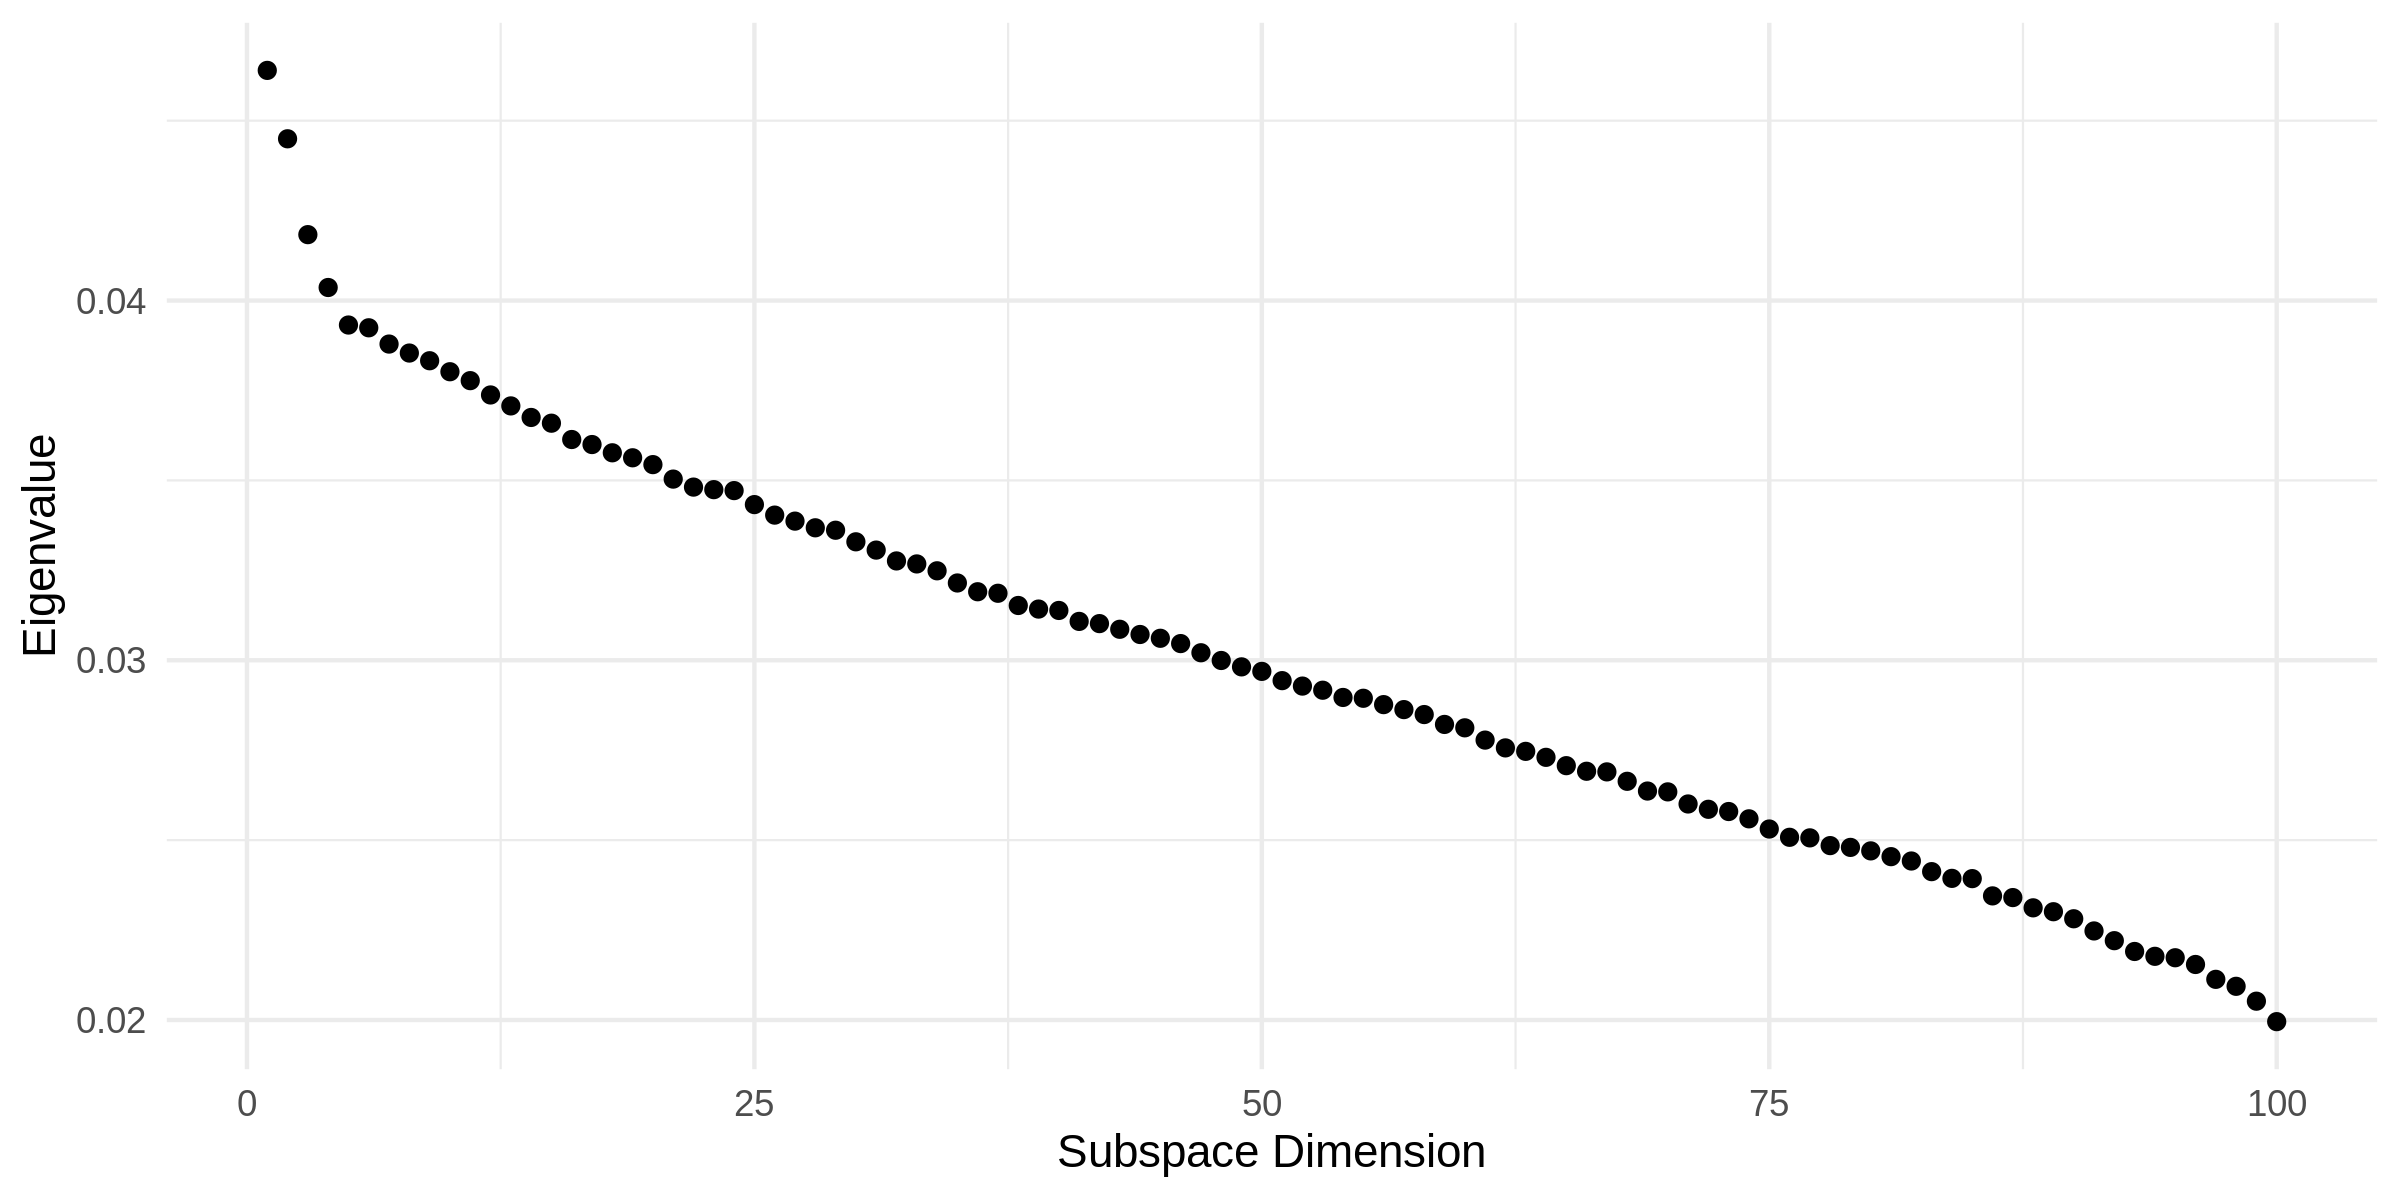
\includegraphics[width=5in]{figures/sim1_ev.png}
    \caption{Caption}
    \label{fig:sim1_ev}
\end{figure}


% \begin{figure*}[t!]
%     \centering
%     \begin{subfigure}[t]{0.45\textwidth}
%         \centering
%         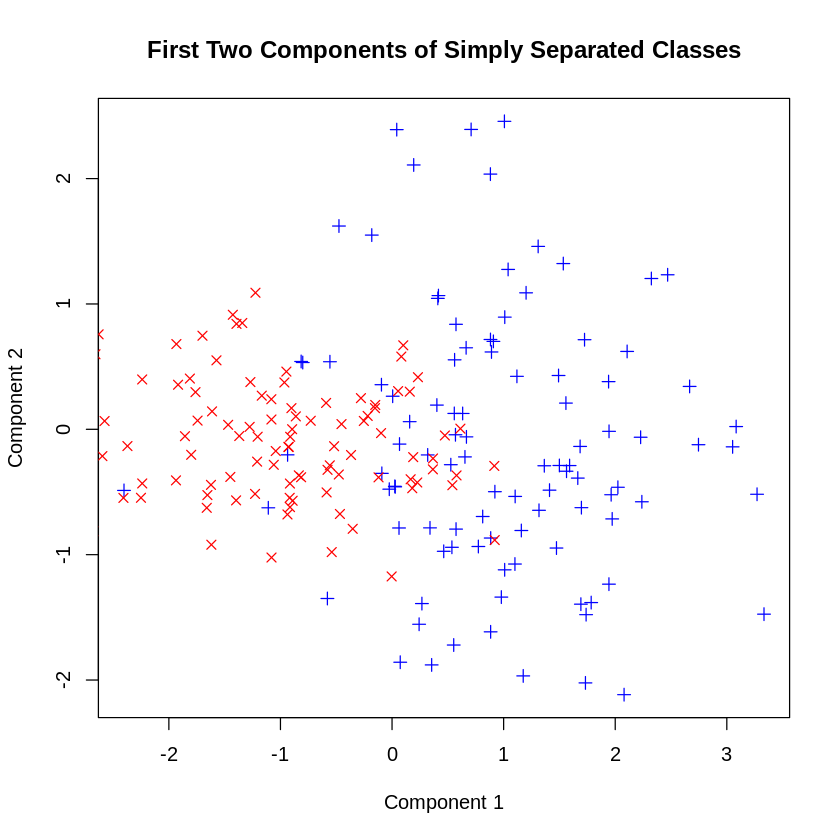
\includegraphics[height=2.3in]{figures/simpleboundary.png}
%         \caption{The distribution of the two classes in the first two components. All other components are identically distributed between the two classes.\label{fig:simpleboundary}}
%     \end{subfigure}%
    
%     \begin{subfigure}[t]{0.45\textwidth}
%         \centering
%         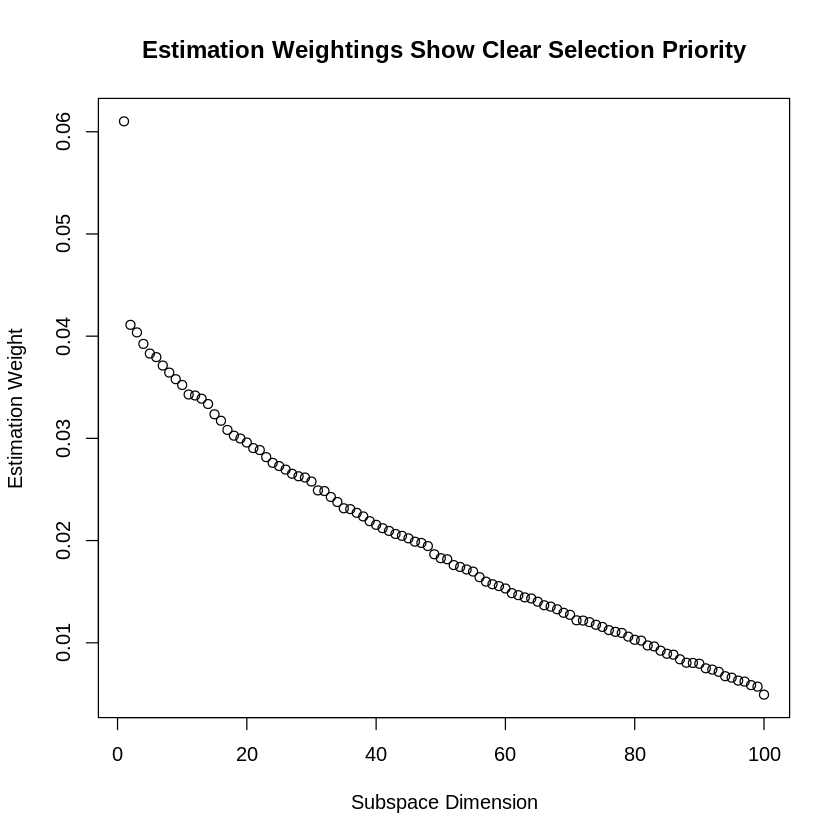
\includegraphics[height=2.3in]{figures/simpleeigs.png}
%         \caption{The sequence of average projection eigenvalues show a clear distinction for the very first basis vector.}
%     \end{subfigure}
%     ~ 
%     \begin{subfigure}[t]{0.45\textwidth}
%         \centering
%         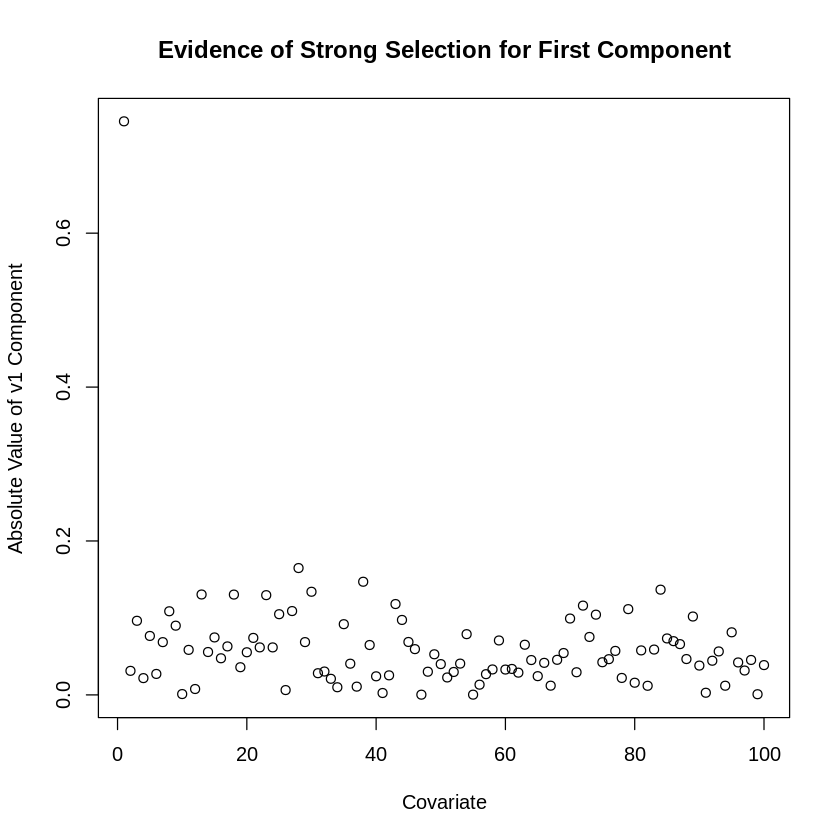
\includegraphics[height=2.3in]{figures/simplecomponents.png}
%         \caption{Investigating the basis vector corresponding to the distinct eigenvalue shows a strong selection for the first component.}
%     \end{subfigure}
% \caption{}
% \end{figure*}


\subsection{Rotated sparse normal}

\begin{figure}
    \centering
    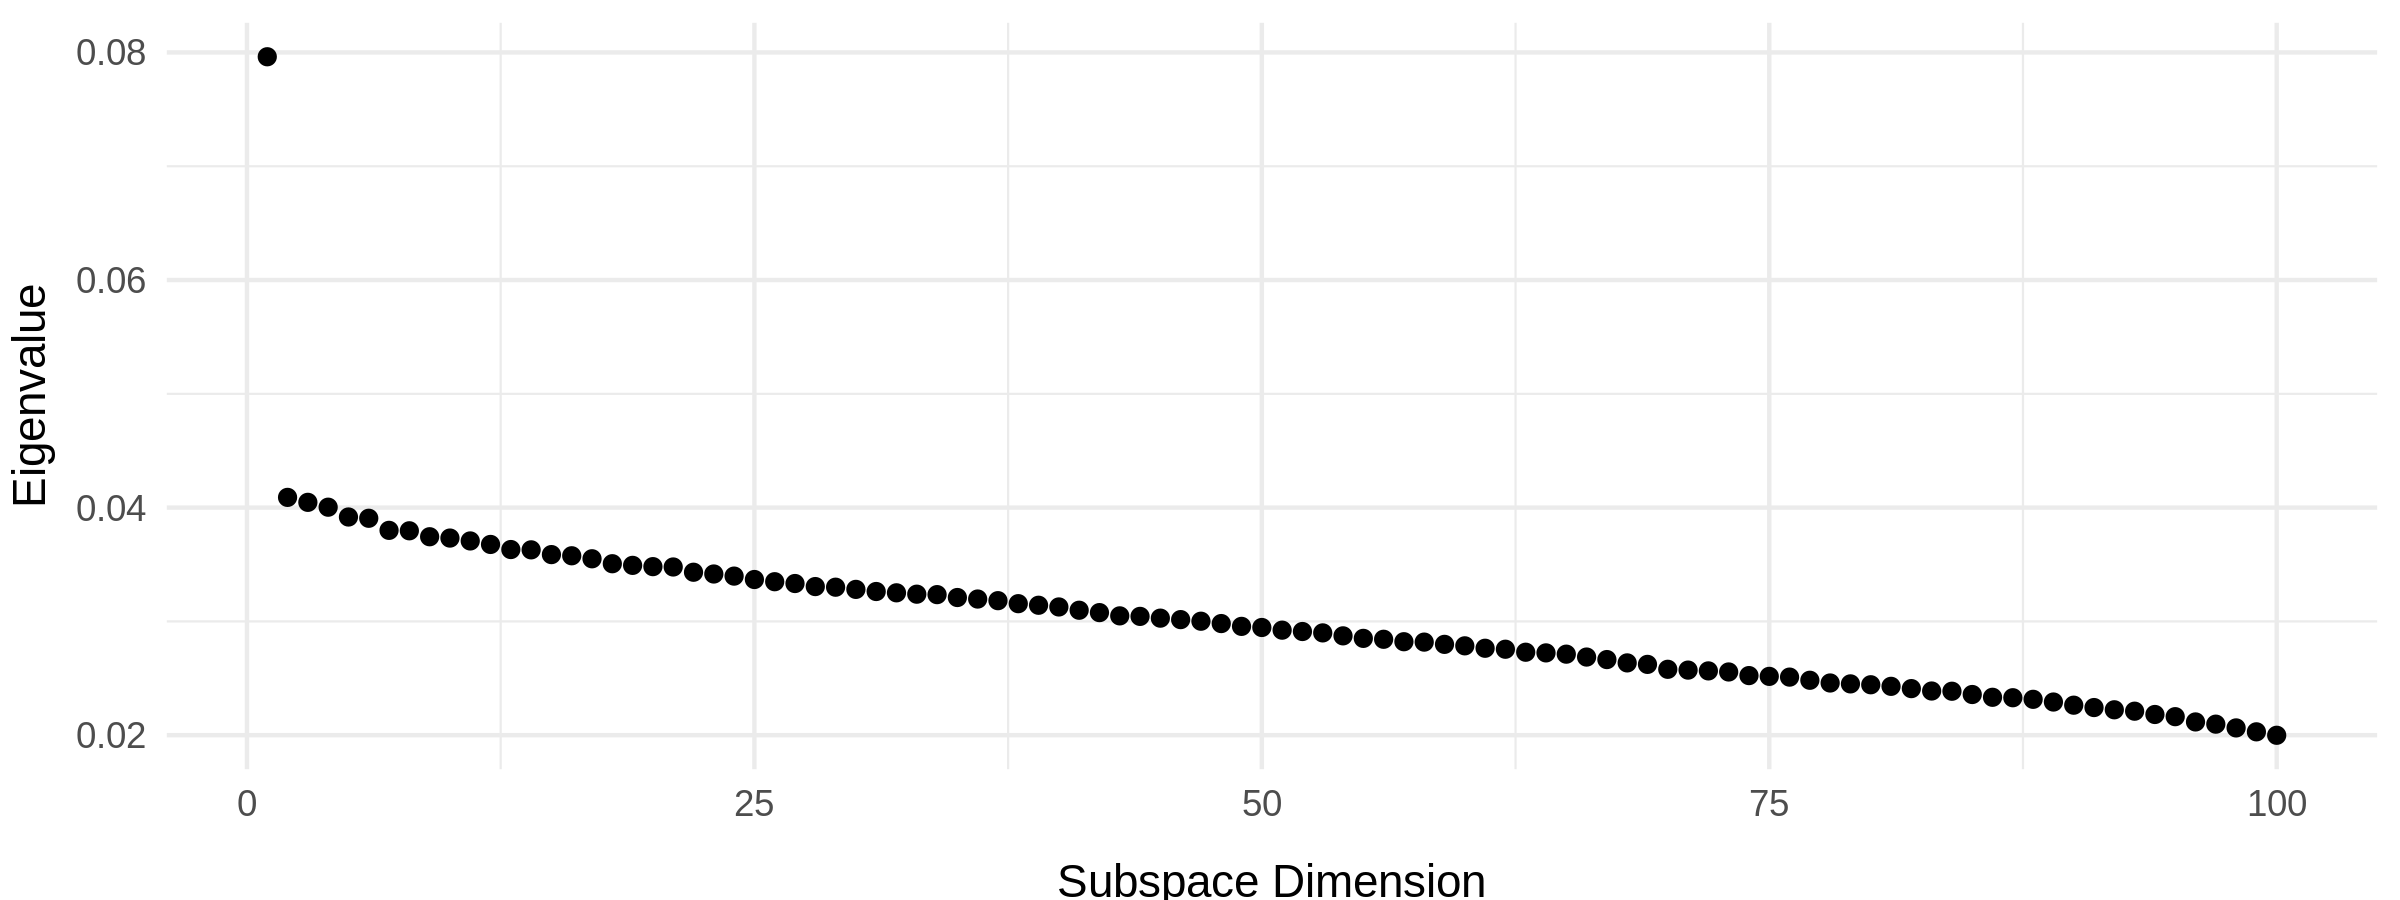
\includegraphics{figures/sim2_ev.png}
    \caption{Caption}
    \label{fig:sim2_ev}
\end{figure}

% \begin{figure*}[t!]
%     \centering
%     \begin{subfigure}[t]{0.45\textwidth}
%         \centering
%         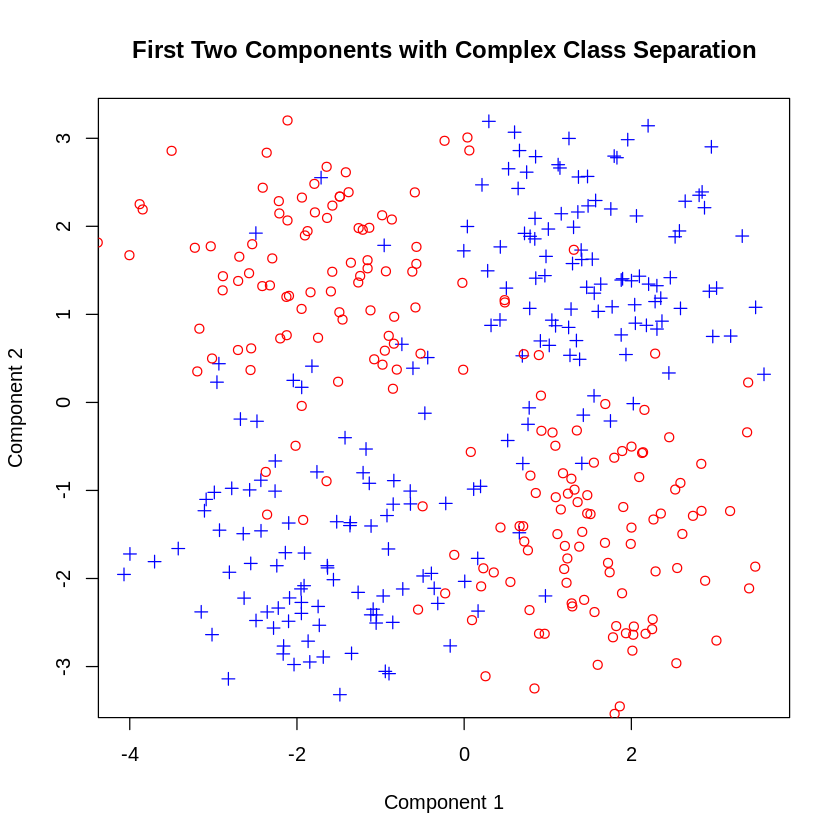
\includegraphics[height=2.2in]{figures/complexboundary.png}
%         \caption{}
%     \end{subfigure}%
%     ~
%     \begin{subfigure}[t]{0.45\textwidth}
%         \centering
%         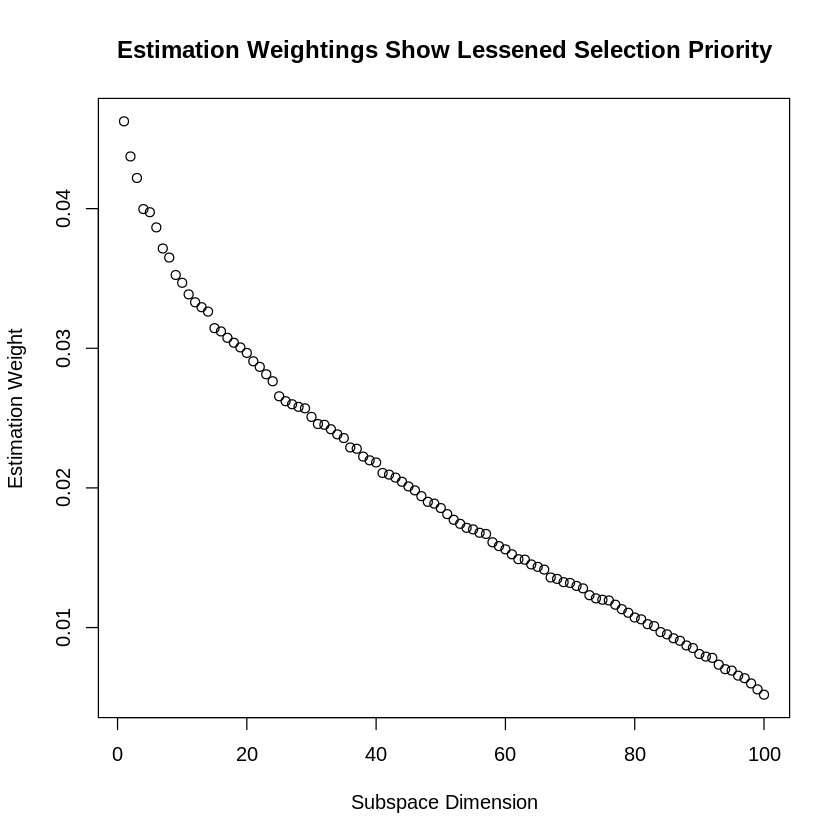
\includegraphics[height=2.2in]{figures/complexeigs.png}
%         \caption{}
%     \end{subfigure}

%     \begin{subfigure}[t]{0.45\textwidth}
%         \centering
%         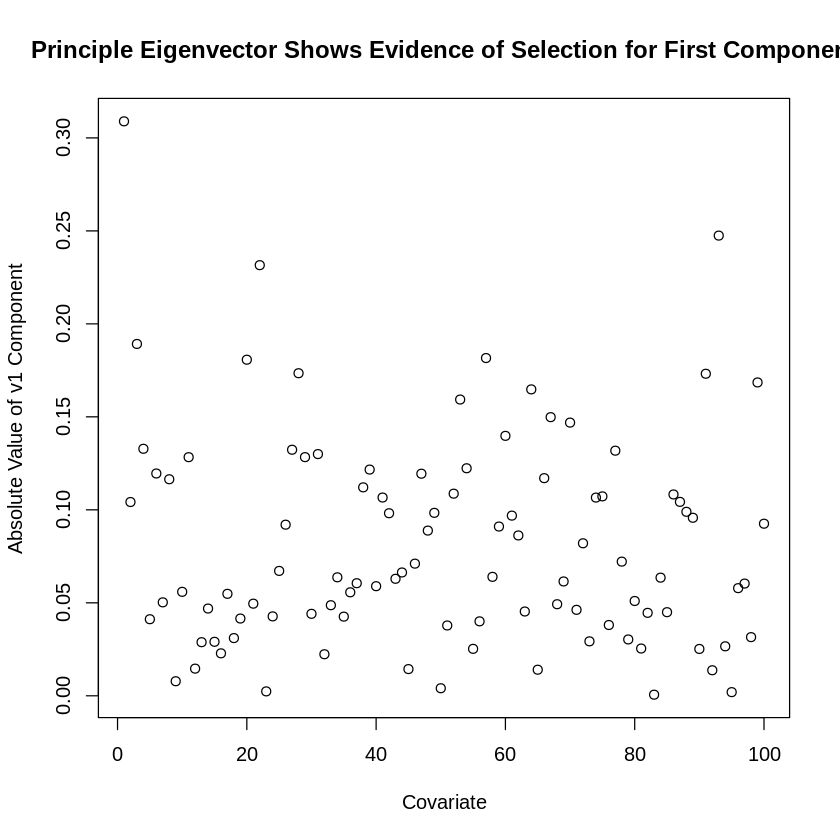
\includegraphics[height=2.2in]{figures/complexfirst.png}
%         \caption{}
%     \end{subfigure}
%     ~
%     \begin{subfigure}[t]{0.45\textwidth}
%         \centering
%         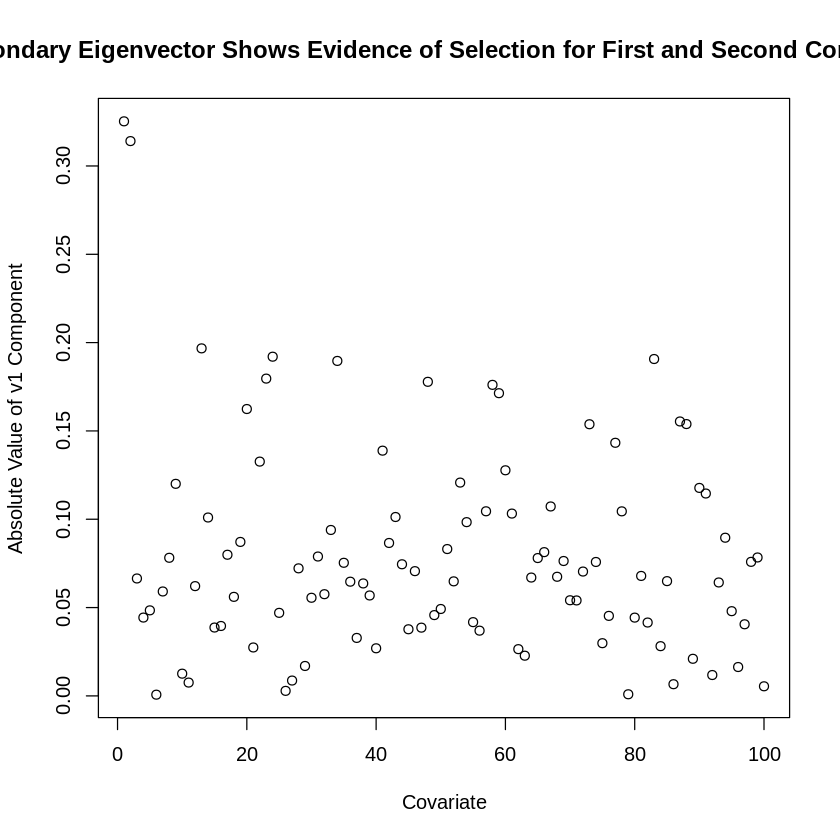
\includegraphics[height=2.2in]{figures/complexsecond.png}
%         \caption{}
%     \end{subfigure}
% \caption{}
% \end{figure*}

\subsection{Independent features}

\begin{figure}
    \centering
    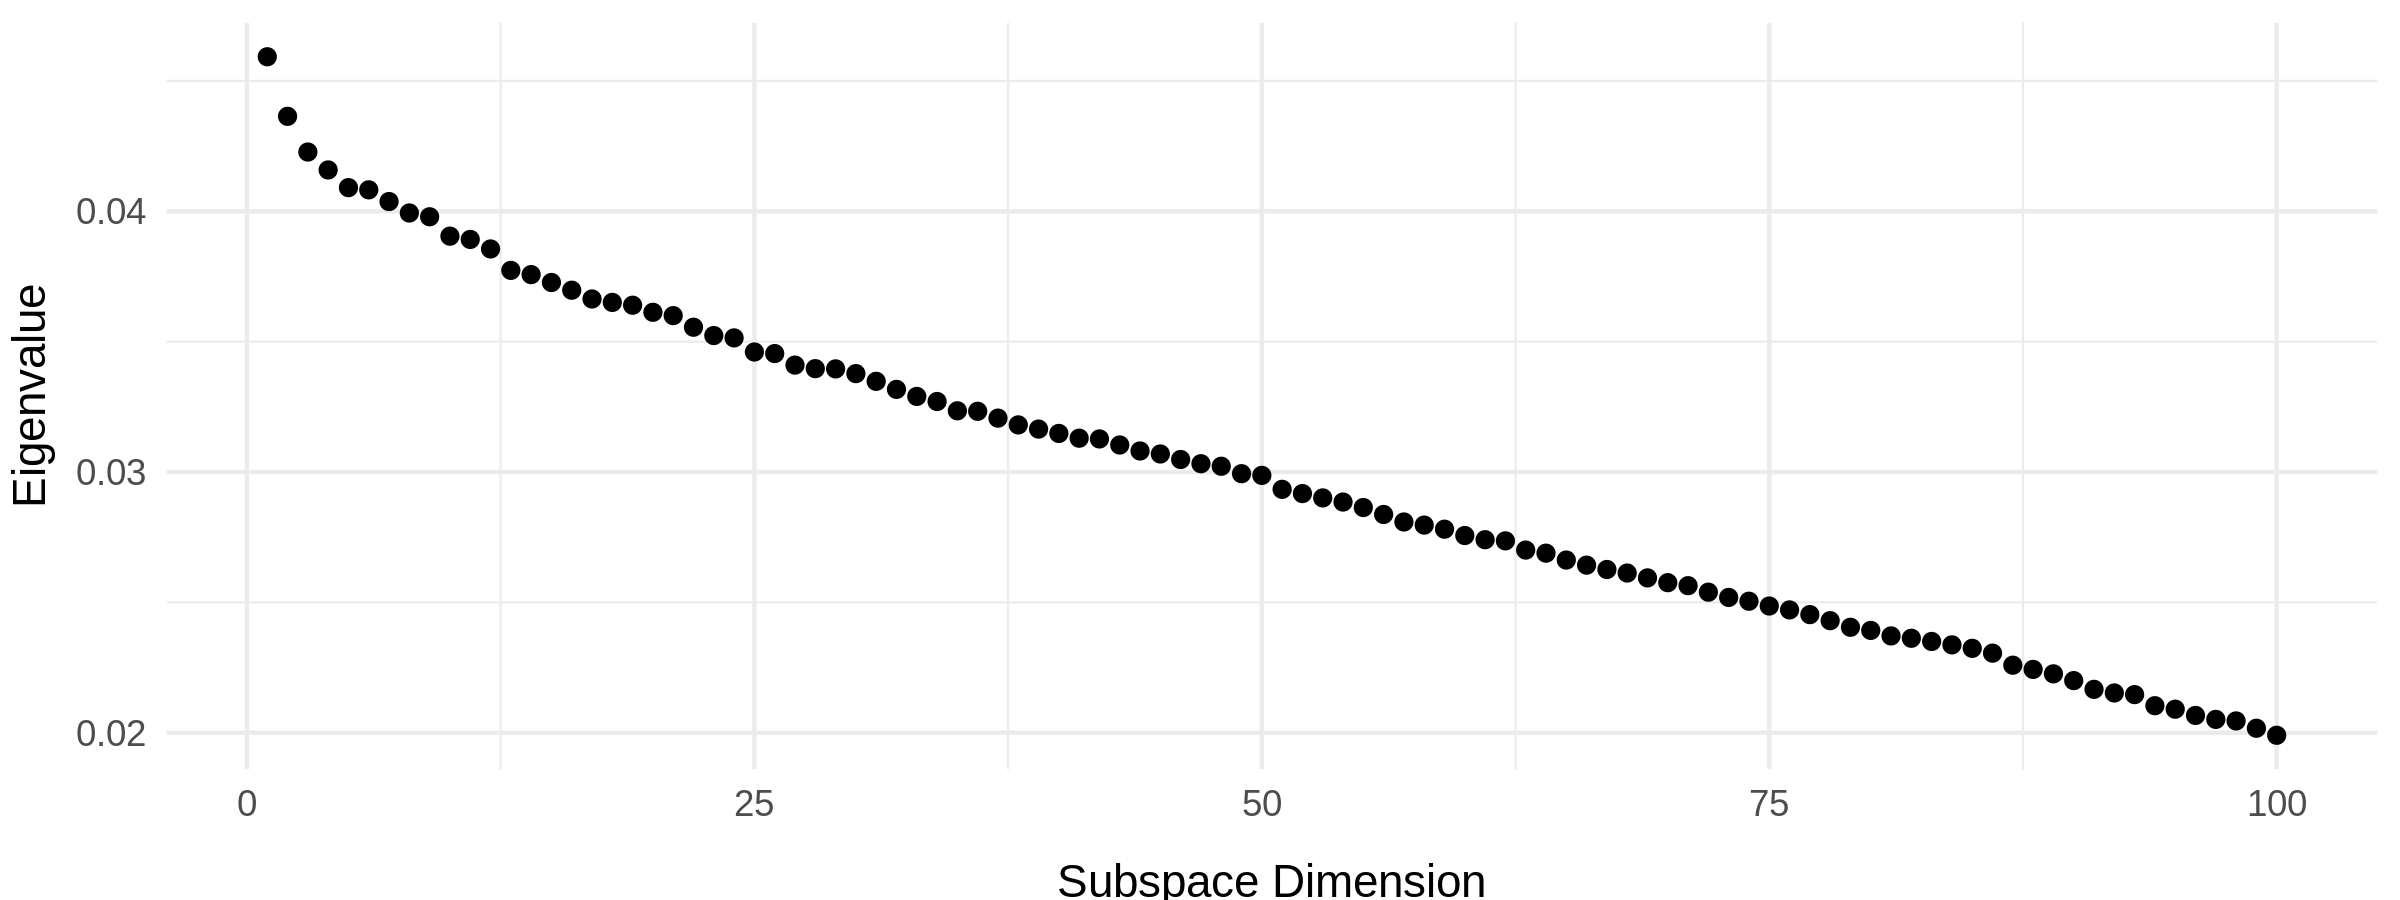
\includegraphics{figures/sim3_ev.png}[]
    \caption{Caption}
    \label{fig:sim3_ev}
\end{figure}

\subsection{$t$‐distributed features}

\begin{figure}
    \centering
    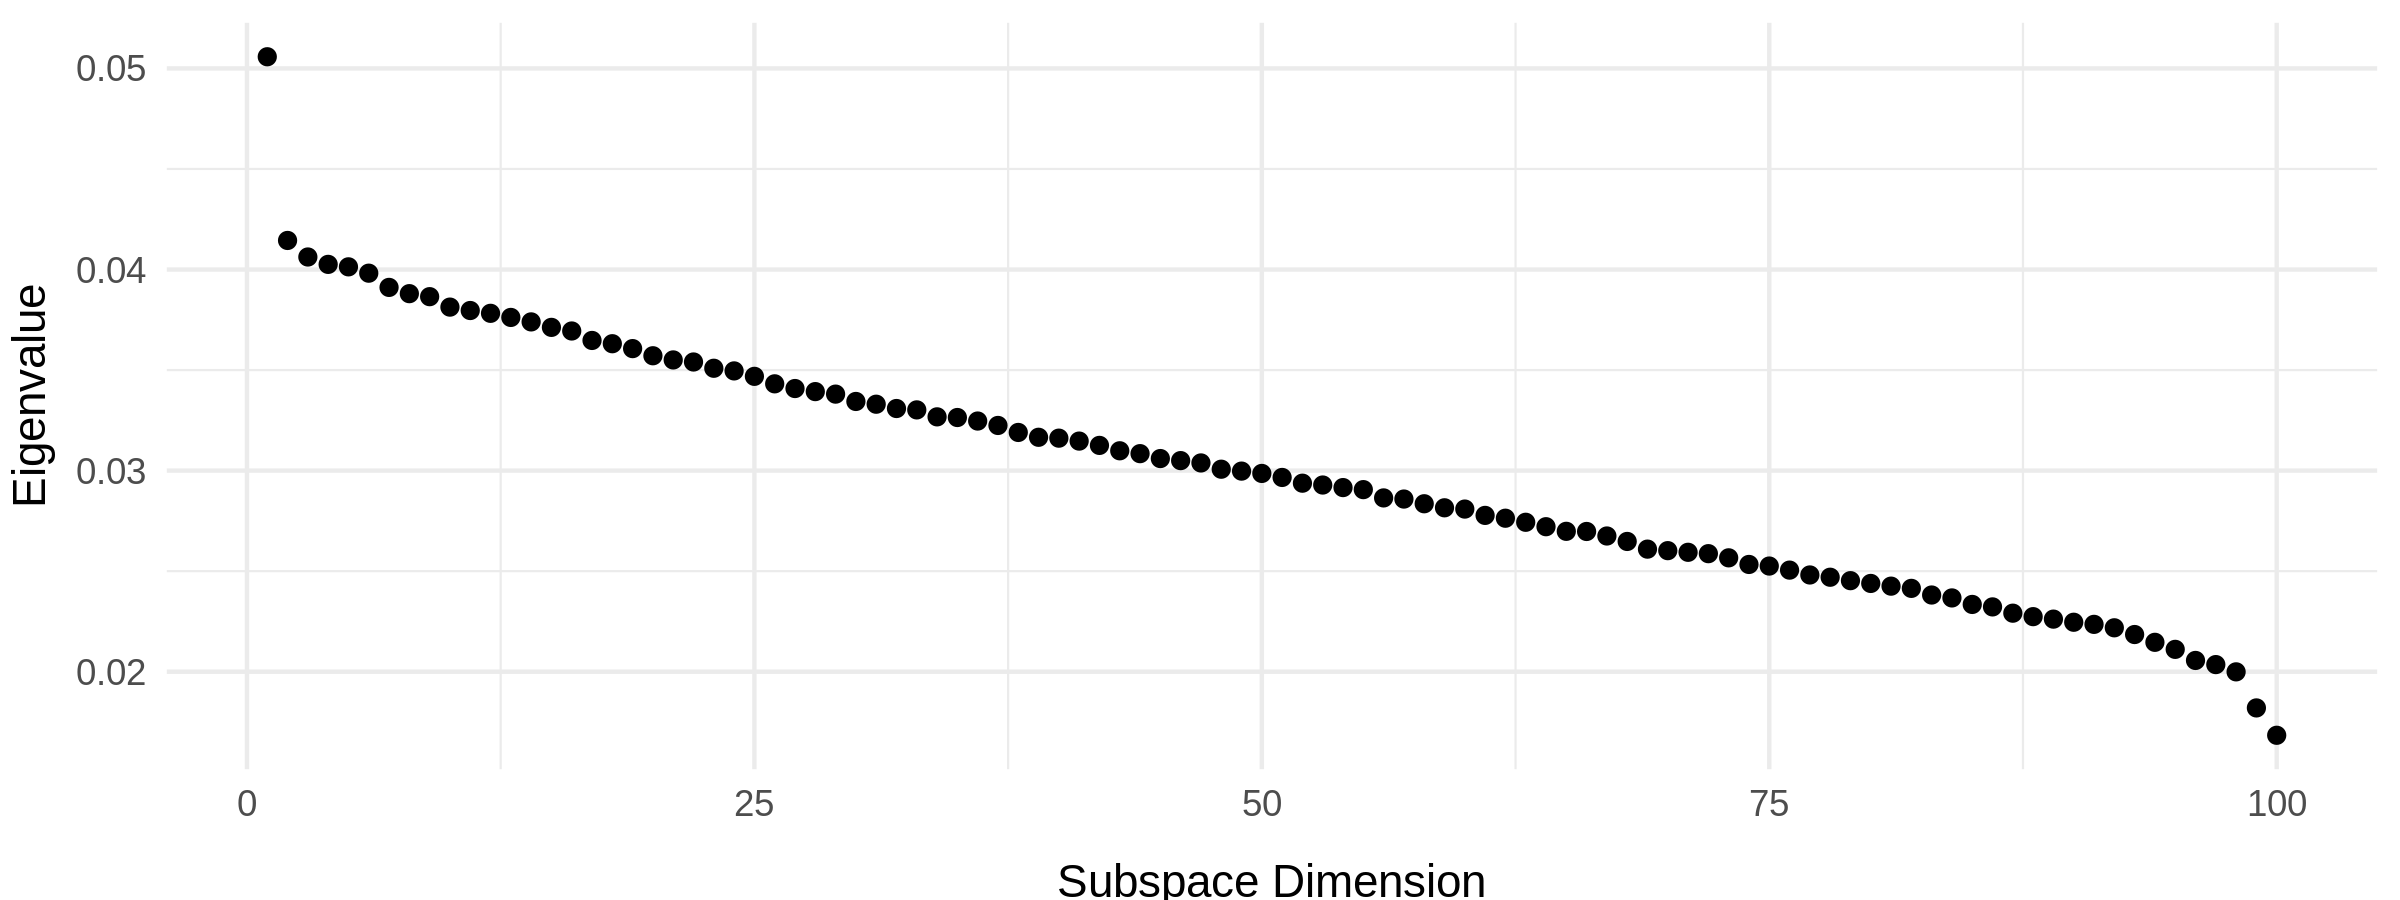
\includegraphics{figures/sim4_ev.png}
    \caption{Caption}
    \label{fig:sim4_ev}
\end{figure}

\section{Real-World Examples}

\subsection{Epilepsy Dataset}


% \section{Generalised formulation?}
% If we made good progress on the techniques that we've got at the moment, I think there would be scope for looking at a range of generalisations. These can be grouped into alterations of the selection method for choosing random projections, and alterations of the distance measure used to obtain low-dimensional representations. Consider the following (very general) setup, where we have a few objects:
% \begin{itemize}
%     \item A training set $\mathcal{T}_n$.
%     \item A collection of projections $\mathcal{A} := \{ A_b \in \mathbb{R}^{d\times p} : b \in \{ 1,\dots,B\}$ (by projections we mean that for all $b$, $A_bA_b^T = I_d$).
%     \item A base classifier, i.e. a map $C : (\mathcal{T}_n, A) \mapsto C^A_{\mathcal{T}_n}$ where $C^A_{\mathcal{T}_n}$ is a function $C^A_{\mathcal{T}_n}: \mathcal{X} \rightarrow \mathcal{Y}$.
%     \item A selection procedure, by which we mean a map $s : (\mathcal{T}_n, \mathcal{A}, b, C) \mapsto s_b$ where $s_b:\mathcal{X}^2 \rightarrow \{0,1\}$ is a function detailing which pairs of observations to select that projection for. 
%     \item A positive definite kernel $k: \mathbb{R}^d \times \mathbb{R}^d \rightarrow \mathbb{R}$.
% \end{itemize}

% Now we define a learned distance 

% \[K^\mathcal{A}_{\mathcal{T}_n}(x,x') = \sum_{b: s_b(x,x') = 1} k(A_bx, A_bx').\]

\section*{Appendix}


\bibliographystyle{plainnat}
\bibliography{references.bib}


\end{document}
